\documentclass[a4paper,11pt]{article}
\title{GUIssing game}
\author{Izaak van Dongen}

\usepackage{mysty}

\begin{document}
    \maketitle\thispagestyle{empty} % no page number under title
    \tableofcontents
    \listoflistings

    \section{Introduction}

    This project is the sequel to the popular \texttt{assignment\_guessing}, at
    \url{https://github.com/goedel-gang/assignment_guessing}, now featuring a
    very useful and fluid graphical interface, more object orientation, and
    cleaner general coding practice.

    It uses the same techniques to search both \(\mathbb{Q}\) and
    \(\mathbb{Z}\), but doesn't implement the linear approach to either, as it's
    not really preferable in any circumstance.

    \section{Programs}

    \subsection{Interesting}

    Despite the fact that the same algorithms from last time can be reapplied,
    their implementations have to be suited the the event-driven idiom. This is
    reflected in listing \ref{lst:guesser}, which contains the `boilerplate'
    code. It represents the broad protocol that a component implementing
    guessing should follow.

    This is that a guesser may must implement a method to ask a question, and a
    separate method that receives the answer. The guesser should appropriately
    modify its internal state so that it knows what question is being answered,
    and what to ask next. This is really a kind of poor man's synchronous
    coroutine, as implemented for example by Python's generators, where the
    internal state is simply a stack frame. However, these do not come with fpc.

    The other thing to note is that a guesser being able to deduce a number is
    considered exceptional behaviour, and hence is implemented by an exception,
    which should carry a message including what the correctly guessed number is,
    which may then be caught. If the guesser is not sure of the user's number,
    it should simply ask a normal question to verify if a guess is correct. This
    is implemented for example in listing \ref{lst:sternbrocot}.

    It is implemented as an abstract class rather than as an interface because
    the main code also wants to be able to tear the engine down, with a
    \texttt{Free} call to prevent memory leakage. Unfortunately, destructors
    can't be included in interfaces, so there is no guarantee that an
    implementing class can be freed. Because of this, I instead use an object,
    which \textit{is} understood to have a \texttt{Free} method.

\begin{longlisting}
\inputminted{Pascal}{../UGuesser.pas}
\caption{UGuesser.pas: Boilerplate and definitions for guessing objects}
\label{lst:guesser}
\end{longlisting}

    Listing \ref{lst:binary} shows a class implementing this protocol, namely by
    performing a binary search. As previously discussed, this version of binary
    search works on the entirety of \(\mathbb{Z}\), by determining bounds in a
    similar `binary' manner (at least, it should be able to find sensible bounds
    in \(\BigO(\log_2(n))\) (and then guess the number in \(\BigO(\log_2(n))\)).

\begin{longlisting}
\inputminted{Pascal}{../UBinarySearch.pas}
\caption{UBinarySearch.pas: Implementation of unbounded binary search}
\label{lst:binary}
\end{longlisting}

    Listing \ref{lst:sternbrocot} shows a class implementing a search on
    \(\mathbb{Q}\). This is separated from listing \ref{lst:binary} as when
    considering the case of integers, this effectively degenerates into a slow
    linear search (taking the consecutive upper mediants of \(\frac{0}{1}\) and
    \(\frac{1}{0}\) results in the sequence \(\frac{1}{1}\), \(\frac{2}{1}\),
    \(\frac{3}{1}\)\ldots).

\begin{longlisting}
\inputminted{Pascal}{../USternBrocotSearch.pas}
\caption{USternBrocotSearch.pas: Implementation of unbounded rational search}
\label{lst:sternbrocot}
\end{longlisting}

    Listing \ref{lst:dummy} shows a dummy class that just displays a message
    whenever it is queried. This is useful for the main form code to show a
    persistent message to the user while no other searching engine is
    instantiated.

\begin{longlisting}
\inputminted{Pascal}{../UDummyGuesser.pas}
\caption{UDummyGuesser.pas: Dummy message-displaying object}
\label{lst:dummy}
\end{longlisting}


    \subsection{Boring}

    Listings \ref{lst:complfm} and \ref{lst:usrlfm} contains abridged versions
    of the lfm (Lazarus Forms) files, serving as a brief summary of all that I
    did in the object inspector.

\begin{longlisting}
\inputminted{pascal}{UComputerGuessing.lfm}
\caption{(Heavily redacted) UComputerGuessing.lfm: Layout and programmatic
properties of Form elements}
\label{lst:complfm}
\end{longlisting}

\begin{longlisting}
\inputminted{pascal}{UUserGuessing.lfm}
\caption{(Heavily redacted) UUserGuessing.lfm: See \ref{lst:complfm}}
\label{lst:usrlfm}
\end{longlisting}

    Listing \ref{lst:compforms} shows the `main' code that deals with the
    \texttt{TForm}. This part implements all the callbacks specified for each
    form component, and relays the user's actions to the \texttt{TGuesser}
    currently in action.

\begin{longlisting}
\inputminted{Pascal}{../UComputerGuessing.pas}
\caption{UComputerGuessing.pas: Implementing the Forms functionality}
\label{lst:compforms}
\end{longlisting}

    Listing \ref{lst:usrforms} contains similar code but for the mode where the
    user must guess the computer's number. This is perhaps even more mundane as
    really all it does is handle a lot of conversions and check a couple of
    cases.

\begin{longlisting}
\inputminted{Pascal}{../UUserGuessing.pas}
\caption{UUserGuessing.pas: Implementing the Forms functionality}
\label{lst:usrforms}
\end{longlisting}

    My favourite part of the form code is \texttt{KeyIntercept}, which enables
    the user not to have to press any buttons or really use the GUI at all,
    upgrading its usefulness to near CLI levels.

    \section{Result}

    Screenshots of the application are shown in fig \ref{pic:app}. The colouring
    is not specifically set for this game, but is just my personal GTK theme
    (Arc-Dark), which is used as Lazarus implement Forms with GTK2.

\begin{figure}[H]
\begin{center}
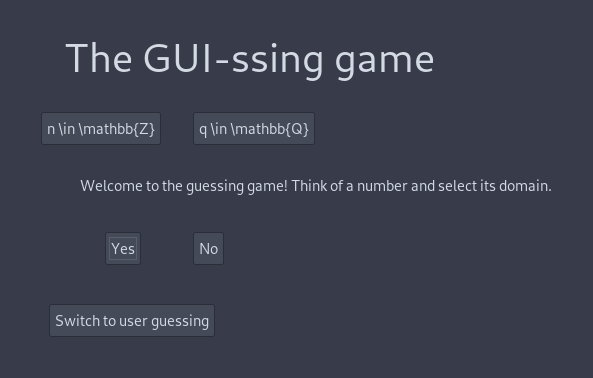
\includegraphics[height=0.2\textheight]{win_screenshot_20180611_202749.png}
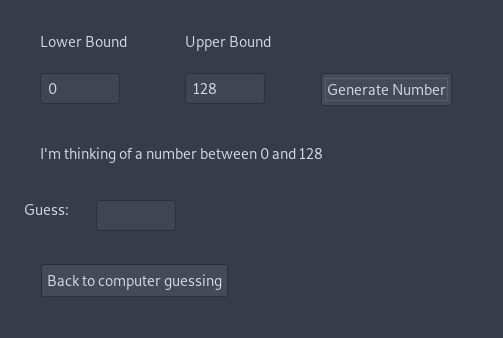
\includegraphics[height=0.2\textheight]{win_screenshot_20180611_202757.png}
\end{center}
\caption{Screenshots of the game}\label{pic:app}
\end{figure}

    You may notice that all of the mathematics is formatted in the form of
    \LaTeX\ source. This is the second best\footnote{For example, it beats
    straight utf-8 because it allows a user to render the maths using whatever
    font they like in their head} way to format maths, beside rendered \LaTeX.

    The program can be interacted with by clicking the buttons, or, as covered
    earlier, by pressing the appropriate keys. I have also chosen
    \texttt{TLabel} to communicate with the user rather than a \texttt{TListBox}
    as it is more compact, and I feel better represents the spirit of a guessing
    game (I consider it a vital component that your internal state should be
    kept in your head, and would be furious if my opponent were to write
    anything down).

    Because of the various \mintinline{pascal}{writeln} statements I had
    included, I can easily capture the actions executed by the user and program
    without needing multiple screenshots. I first compiled using
    \texttt{lazbuild} or Lazarus, and then ran \mintinline{zsh}{./GUIssing >
    writeup/output.txt}. This produced the file in listing \ref{lst:output},
    after I executed a guess for \(\forall S \in \{\mathbb{Z}, \mathbb{Q}\}\).

\begin{longlisting}
\inputminted{text}{output.txt}
\caption{Example log of session with program}\label{lst:output}
\end{longlisting}

    This demonstrates the program correctly feeding information between the user
    and the underlying search engine. I have performed several more tests,
    including the cases

    \begin{tabular}{r *7M}
        in \(\mathbb{Z}\): & 0     & 1     & -1    & 200   & -130  & 16 \\
        in \(\mathbb{Q}\): & 0 & 1 & 3 & -3 & \frac{4}{3} & \frac{5}{2} & -\frac{5}{2} \\
    \end{tabular}

    These were not included as entire logs as this would be a
    serious waste of paper.

    Note that this program will fail if the user decided on a number not
    representible by a Pascal \texttt{integer}, as shown in listing
    \ref{lst:overflow}. To solve this problem permanently would require an
    implementation of some kind of \texttt{BigInteger}. This would require lots
    more memory management and boilerplate, which in turn needs time. I'm
    currently mildly strapped for time so I've opted to let it break.

    This is not a problem for the computer-generated guessing mode as each TEdit
    limits its input to 8 characters, leaving the user to input at largest
    \(10^8-1\). This is well within the range of a signed 32-bit integer
    (\,\(\abs{n} \lessapprox 2.1 \cdot 10^9\)). Another non-bug in this part is
    if the user enters a lower bound larger than the upper bound (let \(a >
    b\)). In this case, a random number in the interval \([a, 2a - b) \cap
    \mathbb{Z}\) is generated. For example, \(a = 100, b = 50\) results in a
    number in \(\{100..149\}\). This is due to the fact that Pascal's
    \texttt{random} function treats its input as an absolute value. This is
    ideal behaviour\footnote{Users trying to mess with the program get messed
    with instead}.

\begin{longlisting}
\begin{minted}{text}
Question: Is 536870912 \le \abs{n} < 1073741824?
Pressed key n
Answer No
Question: Is 1073741824 \le \abs{n} < -2147483648?
Pressed key n
Answer No
Question: Is -2147483648 \le \abs{n} < 0?
Pressed key n
Answer No
Question: Is 0 \le \abs{n} < 0?
Pressed key n
Answer No
Question: Is 0 \le \abs{n} < 0?
\end{minted}
\caption{Overflow leading to critical failure}\label{lst:overflow}
\end{longlisting}

    \section{Source}

    The full project in its directory structure, including this document (as a
    full-colour PDF and \TeX{} file), can be found at
    \url{https://github.com/goedel-gang/GUIssing}.

\end{document}
